\documentclass[10pt]{beamer}
\usepackage[english]{babel}
\usepackage[utf8]{inputenc}
\usepackage[T1]{fontenc}
\usepackage{helvet}
\usepackage{listings}
%-------------------------------------------------------
% INFORMATION IN THE TITLE PAGE
%-------------------------------------------------------

\newcommand{\cstitle}{\textbf{Mineria de Datos}}
\subtitle[]{DNA sequence similarity analysis using image texture analysis}
\newcommand{\cscourseCode}{1704146}
\newcommand{\csauthor}{MSc. Vicente Machaca Arceda}
%\institute[UNSA]{Universidad Nacional de San Agustín de Arequipa}
\institute[UNSA]{\textbf{UNIVERSIDAD NACIONAL DE SAN AGUSTÍN}}
\newcommand{\csemail}{vmachacaa@unsa.edu.pe}
\newcommand{\instituteabr}{UNSA}
\newcommand{\nameUp}{ICC Fase 1}
\date{\today}
\title[\cscourseCode]{\cstitle}
\author{\csauthor}
%%%%%%%%%%%%%%%%%

%-------------------------------------------------------
% CHOOSE THE THEME
%-------------------------------------------------------
\def\mycmd{0} % CS THEME
\def\mycmd{1} % MYTHEME
%-------------------------------------------------------

\newcommand{\namelogo}{img/2_dna.png}

\if\mycmd1
\usetheme[]{Feather}
\newcommand{\chref}[2]{	\href{#1}{{\usebeamercolor[bg]{Feather}#2}} }
\else
\usepackage{csformat}
\fi

\newcommand{\1}{
	\setbeamertemplate{background}{
		
\includegraphics[width=\paperwidth,height=\paperheight]{img/1_dna}
		\tikz[overlay] \fill[fill opacity=0.75,fill=white] (0,0) rectangle (-\paperwidth,\paperheight);
	}
}


%\usepackage[spanish]{babel}
%\AtBeginDocument{\selectlanguage{spanish}}
%\renewcommand{\figurename}{Figura}
%\renewcommand{\refname}{Referencias}
%\renewcommand{\tablename}{Tabla}



%-------------------------------------------------------
% THE BODY OF THE PRESENTATION
%-------------------------------------------------------

\begin{document}
	
	
\AtBeginSection[]
{
\begin{frame}
\frametitle{Overview}
\tableofcontents[currentsection]
\end{frame}
}


%-------------------------------------------------------
% THE TITLEPAGE
%-------------------------------------------------------

\if\mycmd1 % MY THEME
\1{
\begin{frame}[plain,noframenumbering] 
\titlepage 
\end{frame}}

\else % CS THEME
\maketitle
\fi


%-------------------------------------------------------
%-------------------------------------------------------
\begin{frame}{Overview}
\tableofcontents
\end{frame}
%-------------------------------------------------------
%-------------------------------------------------------




%%%%%%%%%%%%%%%%%%%%%%%%%%%%%%%%%%%%%%%%%%%%%%%%%%%%%%%%%%%%%%%%%%%%%%%%%%%%%%%%%%%%%%%%%%%%%%%%%%%%%%%%%%%%%%%%
%%%%%%%%%%%%%%%%%%%%%%%%%%%%%%%%%%%%%%%%%%%%%%%%%%%%%%%%%%%%%%%%%%%%%%%%%%%%%%%%%%%%%%%%%%%%%%%%%%%%%%%%%%%%%%%%
\section{Introduction}
%%%%%%%%%%%%%%%%%%%%%%%%%%%%%%%%%%%%%%%%%%%%%%%%%%%%%%%%%%%%%%%%%%%%%%%%%%%%%%%%%%%%%%%%%%%%%%%%%%%%%%%%%%%%%%%%
%%%%%%%%%%%%%%%%%%%%%%%%%%%%%%%%%%%%%%%%%%%%%%%%%%%%%%%%%%%%%%%%%%%%%%%%%%%%%%%%%%%%%%%%%%%%%%%%%%%%%%%%%%%%%%%%

%-------------------------------------------------------
%-------------------------------------------------------
\begin{frame}{Introduction}{DNA}
\begin{figure}[]
	\centering
	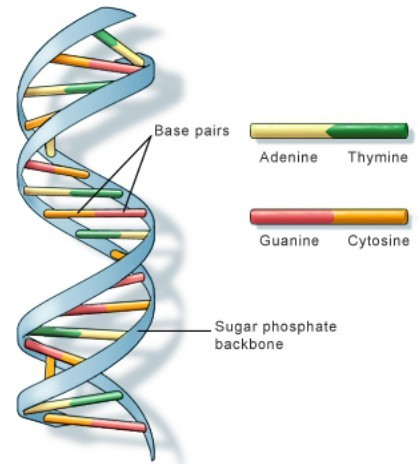
\includegraphics[width=0.5\textwidth,keepaspectratio]{img/mineria/bio6}
	%\label{img:mot2}
	\caption{Molecules in DNA. Adenine, Thymine, Guanine and Cytosine \cite{dna2020located}.}
\end{figure}
\end{frame}
%-------------------------------------------------------
%-------------------------------------------------------


%-------------------------------------------------------
%-------------------------------------------------------
\begin{frame}{Introduction}{DNA}
	\begin{block}{}
		\centering
		The human genome is made of \textbf{\string ~3.2 billions bp} of DNA. \\
		\string ~6.4 billions of nucleotides \cite{archibald2018genomics}.
	\end{block}
	
	\begin{block}{}
		\centering
		The HIV-1 genome is made of \textbf{\string ~20k bp} of DNA. \\
		Meanwhile, the COVID-19 is made of \textbf{\string ~32k bp} \cite{randhawa2020machine}.
	\end{block}	
\end{frame}
%-------------------------------------------------------
%-------------------------------------------------------

%-------------------------------------------------------
%-------------------------------------------------------
\begin{frame}{Introduction}{DNA}
\begin{table}[]
	\caption{Total GigaBytes used to store a complete diploid genome.}
	\begin{tabular}{ll}
		\hline
		DNA bases                & 4           \\
		Bits per base            & 2           \\
		Base pairs per genome    & 3200000000  \\
		Bits per genome          & 12800000000 \\
		Total bits Diplod genome & 25600000000 \\
		Total Kilobytes          & 3125000     \\
		Total Megabytes          & 3052        \\
		\hline
		\textbf{Total Gigabytes}          & \textbf{2.980}      \\
		\hline
	\end{tabular}
\end{table}
\end{frame}
%-------------------------------------------------------
%-------------------------------------------------------

%-------------------------------------------------------
%-------------------------------------------------------
%\begin{frame}{Introduction}{DNA}
%	\begin{figure}[]
%		\centering
%		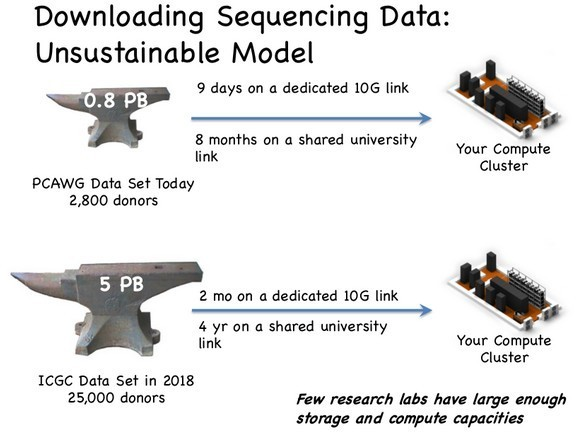
\includegraphics[width=\textwidth,height=0.7\textheight,keepaspectratio]{img/mineria/dat.jpg}
%		\label{img:mot2}
%		\caption{Downloading sequencing data}
%	\end{figure}
%\end{frame}
%-------------------------------------------------------
%-------------------------------------------------------




%-------------------------------------------------------
%-------------------------------------------------------
\begin{frame}{Introduction}{Visualization}
	\begin{figure}[]
		\centering
		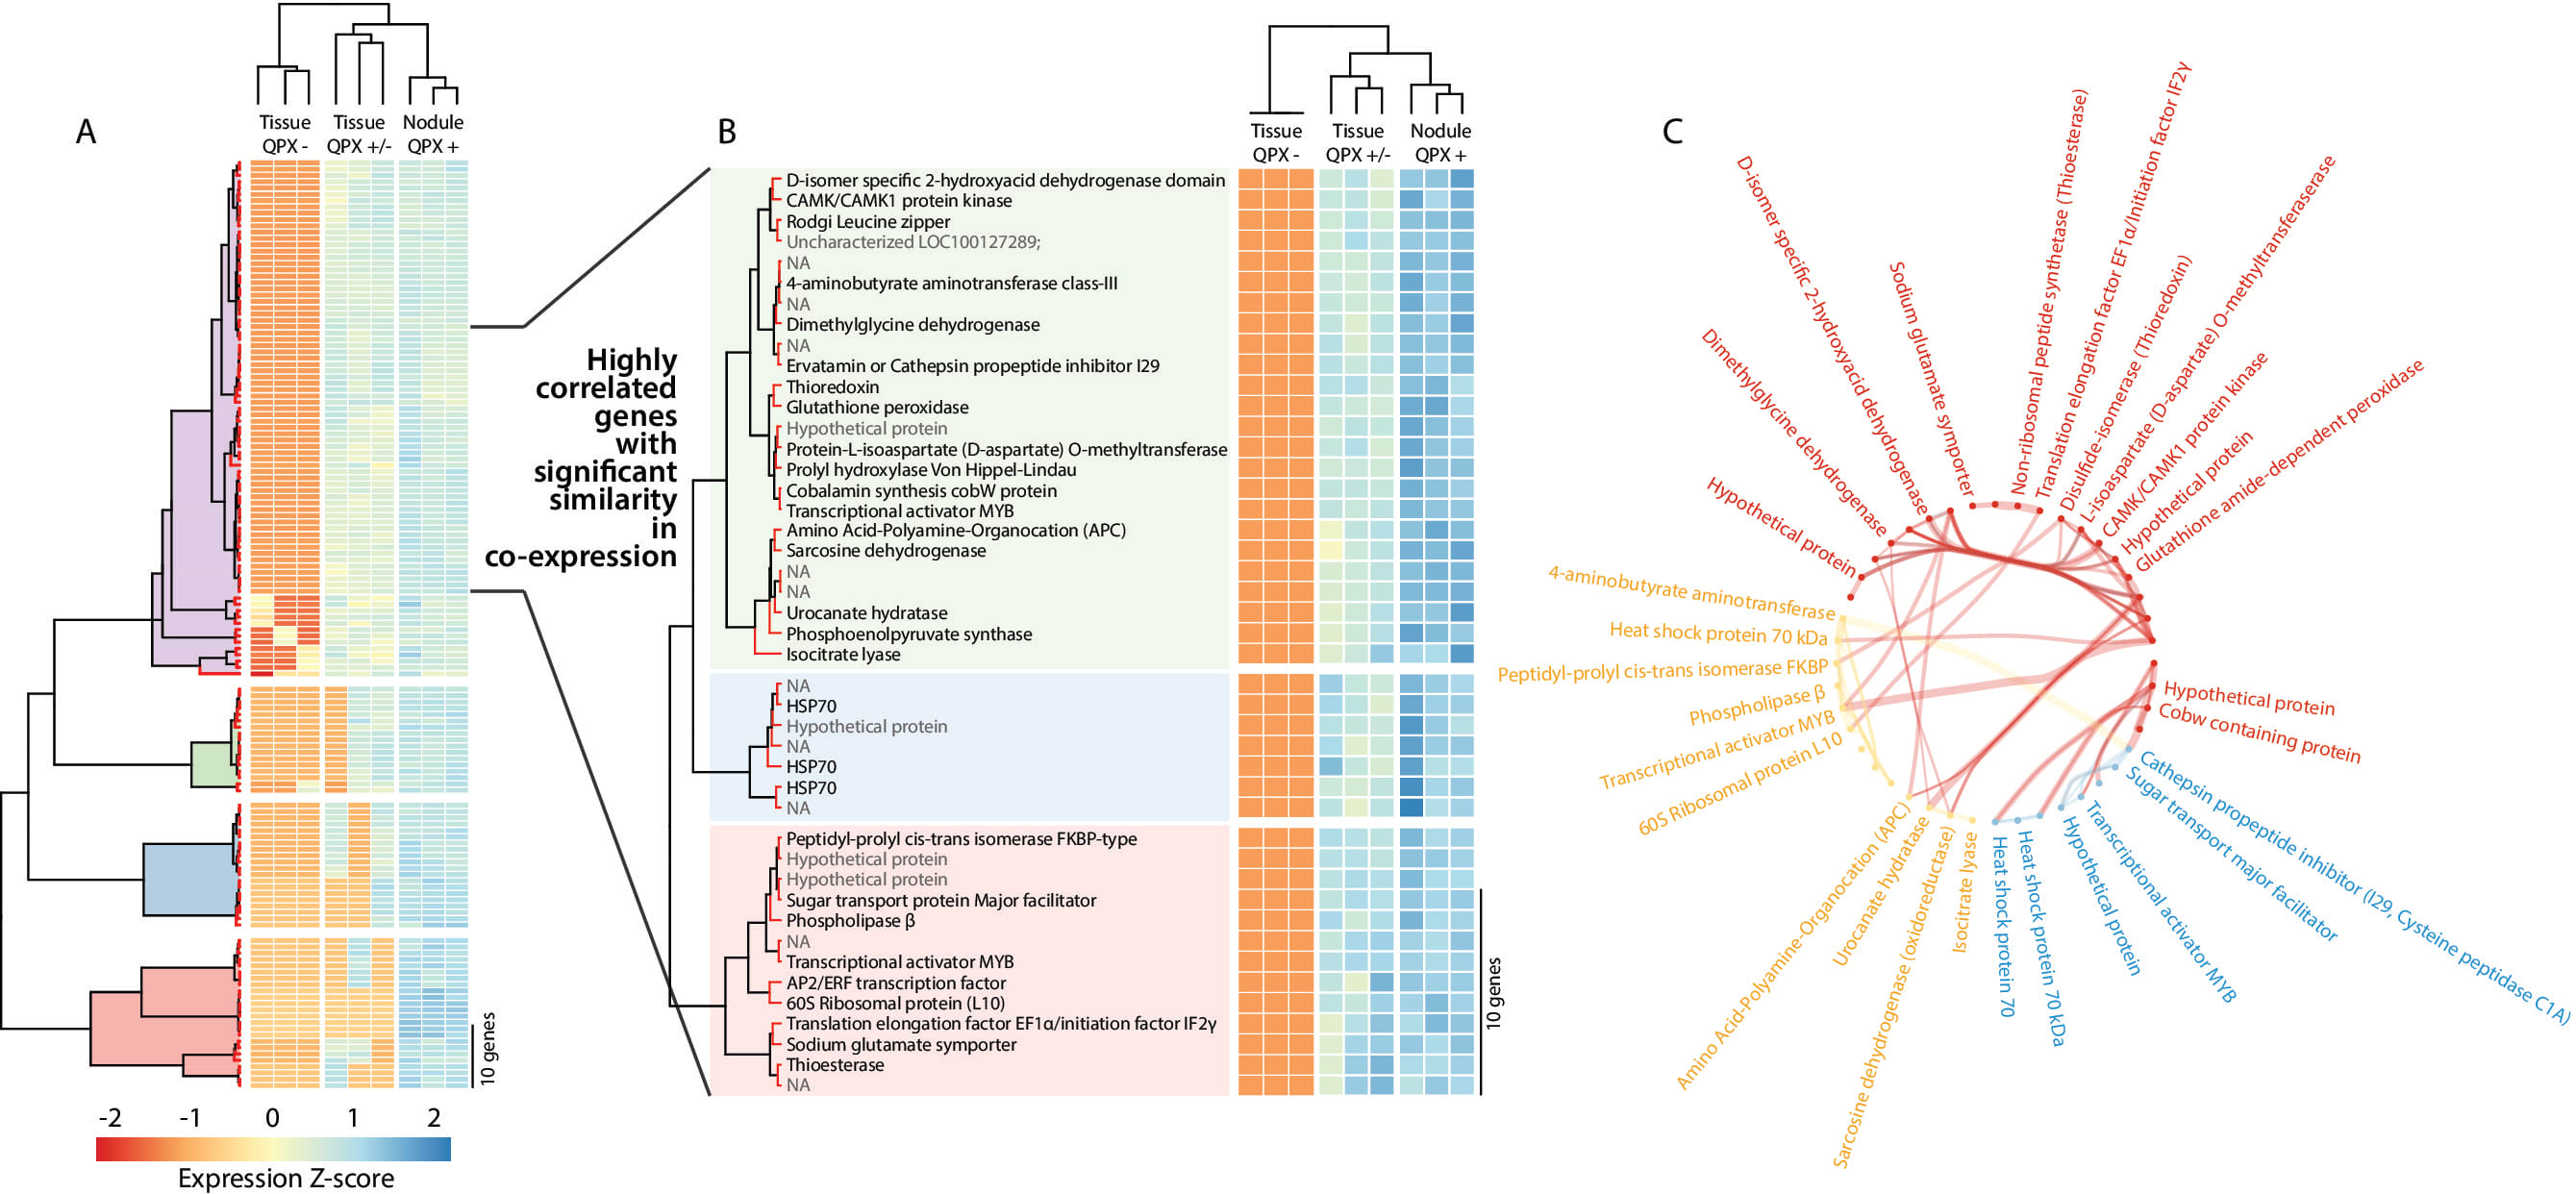
\includegraphics[width=\textwidth,keepaspectratio]{img/mineria/dna_visualization.jpg}
		\label{img:mot2}
		\caption{Example of visualization in bioinformatics.}
	\end{figure}
\end{frame}
%-------------------------------------------------------
%-------------------------------------------------------


%-------------------------------------------------------
%-------------------------------------------------------
\begin{frame}{Introduction}{Similarity and Phylogenetics}
	\begin{block}{Similarity}
		It is used for identifying evolutionary or affinity relations \cite{delibacs2020dna}. Similarity analysis is an important research area in Bioinformatics \cite{jin2017similarity}.
	\end{block}
	
	\begin{block}{Phylogenetics}
		Phylogenetics is the study of the evolutionary history of living organisms using tree-
		like diagrams to represent pedigrees of these organisms \cite{xiong2006essential}.
	\end{block}
\end{frame}
%-------------------------------------------------------
%-------------------------------------------------------

%-------------------------------------------------------
%-------------------------------------------------------
\begin{frame}{Introduction}{Phylogenetics}
	\begin{figure}[]
		\centering
		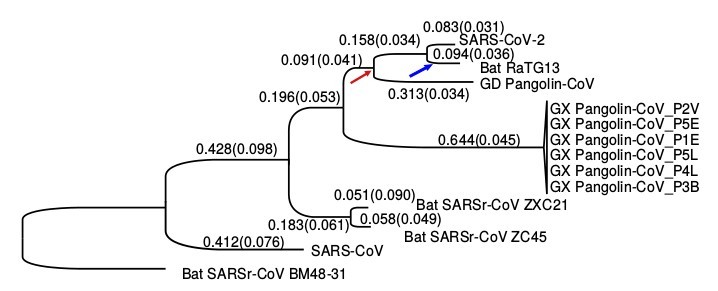
\includegraphics[width=\textwidth,height=0.7\textheight,keepaspectratio]{img/mineria/phylocovid.jpg}
		\label{img:mot2}
		\caption{The phylogenetic tree of SARS-CoV-2 (COVID-19) and the related Coronaviruses  \cite{tang2020origin}.}
	\end{figure}
\end{frame}
%-------------------------------------------------------
%-------------------------------------------------------

%-------------------------------------------------------
%-------------------------------------------------------
\begin{frame}{Introduction}{Phylogenetics}
	\begin{figure}[]
		\centering
		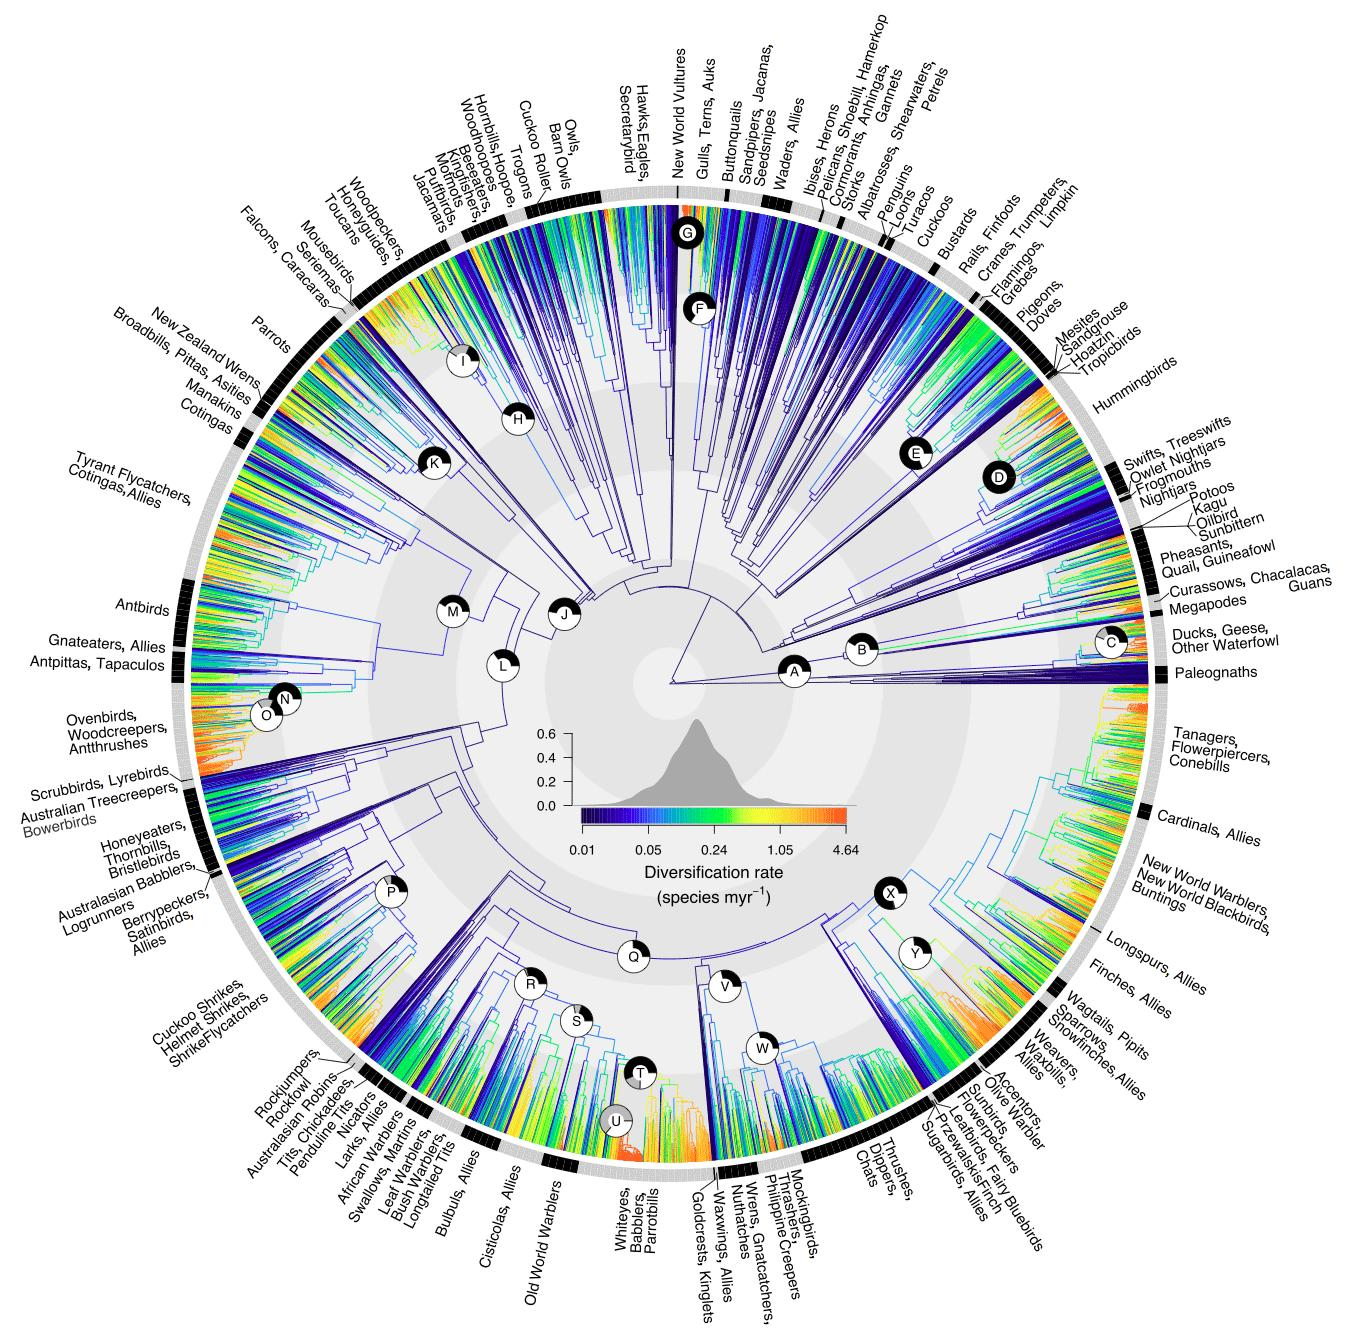
\includegraphics[width=\textwidth,height=0.7\textheight,keepaspectratio]{img/mineria/phylo.jpg}
		\label{img:mot2}
		\caption{The phylogeny tree of bird species  \cite{phylobirds2020}.}
	\end{figure}
\end{frame}
%-------------------------------------------------------
%-------------------------------------------------------





%%%%%%%%%%%%%%%%%%%%%%%%%%%%%%%%%%%%%%%%%%%%%%%%%%%%%%%%%%%%%%%%%%%%%%%%%%%%%%%%%%%%%%%%%%%%%%%%%%%%%%%%%%%%%%%%
%%%%%%%%%%%%%%%%%%%%%%%%%%%%%%%%%%%%%%%%%%%%%%%%%%%%%%%%%%%%%%%%%%%%%%%%%%%%%%%%%%%%%%%%%%%%%%%%%%%%%%%%%%%%%%%%
\section{Problem}
%%%%%%%%%%%%%%%%%%%%%%%%%%%%%%%%%%%%%%%%%%%%%%%%%%%%%%%%%%%%%%%%%%%%%%%%%%%%%%%%%%%%%%%%%%%%%%%%%%%%%%%%%%%%%%%%
%%%%%%%%%%%%%%%%%%%%%%%%%%%%%%%%%%%%%%%%%%%%%%%%%%%%%%%%%%%%%%%%%%%%%%%%%%%%%%%%%%%%%%%%%%%%%%%%%%%%%%%%%%%%%%%%

%-------------------------------------------------------
%-------------------------------------------------------
\begin{frame}{Problem}{Phylogenetics steps}
	\begin{figure}[]
		\centering
		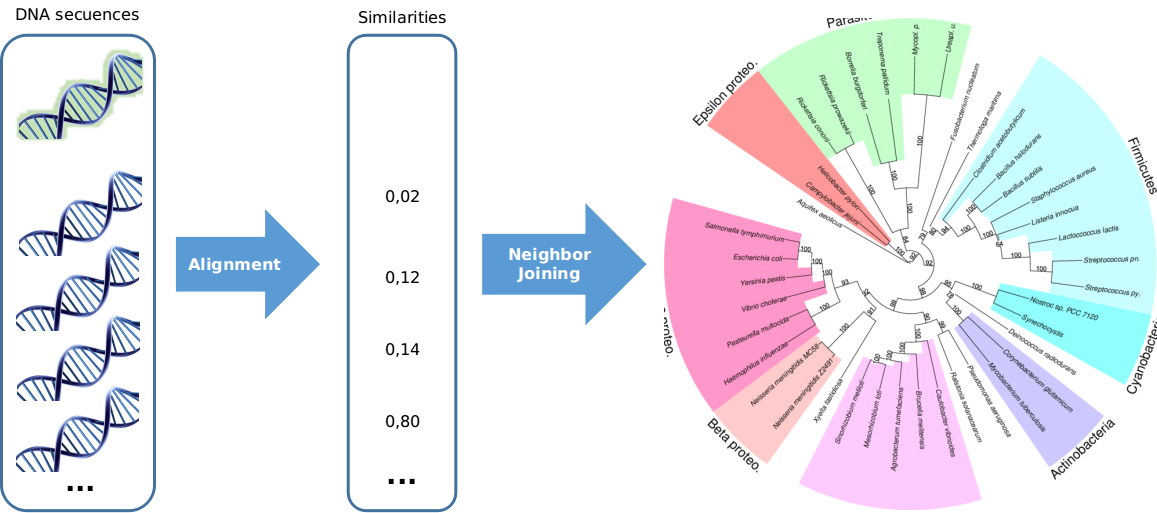
\includegraphics[width=\textwidth,height=0.7\textheight,keepaspectratio]{img/mineria/phylo2}
		\label{img:mot2}
		\caption{Steps to visualize phylonetics trees.}
	\end{figure}
\end{frame}
%-------------------------------------------------------
%-------------------------------------------------------

%-------------------------------------------------------
%-------------------------------------------------------
\begin{frame}{Problem}{Phylogenetics steps}
	\begin{figure}[]
		\centering
		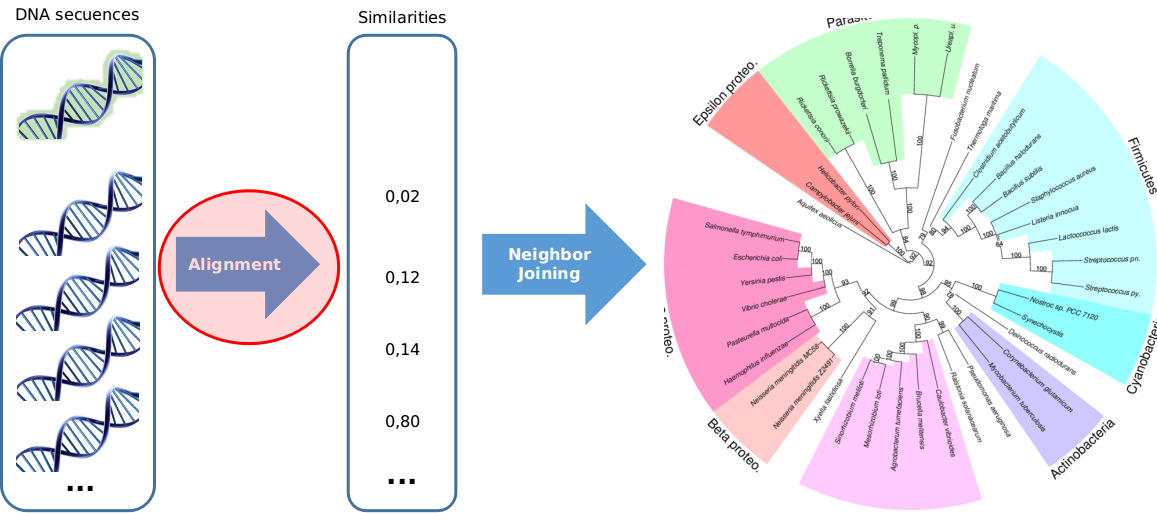
\includegraphics[width=\textwidth,height=0.7\textheight,keepaspectratio]{img/mineria/phylo3}
		\label{img:mot2}
		\caption{Steps to visualize phylonetics trees.}
	\end{figure}
\end{frame}
%-------------------------------------------------------
%-------------------------------------------------------


%-------------------------------------------------------
%-------------------------------------------------------
\begin{frame}{Problem}{Alignment-based methods}
	\begin{block}{}
		\begin{itemize}
			\item The most used \textbf{alignment-based} method is BLAST. \pause
			\item BLAST is slow. \pause
			\item DNA sequences increases every day so BLAST get slower every second. \pause		 	
			\item For example, two days were necessary to build the Phylogenetis tree of COVID-19. 
		\end{itemize}
	\end{block}
\end{frame}
%-------------------------------------------------------
%-------------------------------------------------------

%%%%%%%%%%%%%%%%%%%%%%%%%%%%%%%%%%%%%%%%%%%%%%%%%%%%%%%%%%%%%%%%%%%%%%%%%%%%%%%%%%%%%%%%%%%%%%%%%%%%%%%%%%%%%%%%
%%%%%%%%%%%%%%%%%%%%%%%%%%%%%%%%%%%%%%%%%%%%%%%%%%%%%%%%%%%%%%%%%%%%%%%%%%%%%%%%%%%%%%%%%%%%%%%%%%%%%%%%%%%%%%%%
\section{Proposal}
%%%%%%%%%%%%%%%%%%%%%%%%%%%%%%%%%%%%%%%%%%%%%%%%%%%%%%%%%%%%%%%%%%%%%%%%%%%%%%%%%%%%%%%%%%%%%%%%%%%%%%%%%%%%%%%%
%%%%%%%%%%%%%%%%%%%%%%%%%%%%%%%%%%%%%%%%%%%%%%%%%%%%%%%%%%%%%%%%%%%%%%%%%%%%%%%%%%%%%%%%%%%%%%%%%%%%%%%%%%%%%%%%

%-------------------------------------------------------
%-------------------------------------------------------
\begin{frame}{Proposal}{Objective}
	\begin{block}{}
		Represent the DNA as images and compute textures descriptors in order to get a feature vector. This will reduce time processing in distance processing \cite{delibacs2020dna}. 
	\end{block}

	\begin{block}{}
		Use distances computed before to build phylogenetic trees with \textbf{Evolview v3} (a webserver for visualization, annotation, and management of phylogenetic trees) \cite{subramanian2019evolview}.
	\end{block}
\end{frame}
%-------------------------------------------------------
%-------------------------------------------------------

%-------------------------------------------------------
%-------------------------------------------------------
\begin{frame}{Proposal}{Data}
	\begin{block}{}
	We will use a dataset from beta coronavirus used by Randhawa \cite{randhawa2020machine}. Moreover, the sequences are stored at:
	\begin{itemize}
		\item NCBI.
		\item Virus-host DB
	\end{itemize}
	\end{block}
\end{frame}
%-------------------------------------------------------
%-------------------------------------------------------

%-------------------------------------------------------
%-------------------------------------------------------
%\begin{frame}{Proposal}{Visualization}

%	\begin{figure}[]
%		\centering
%		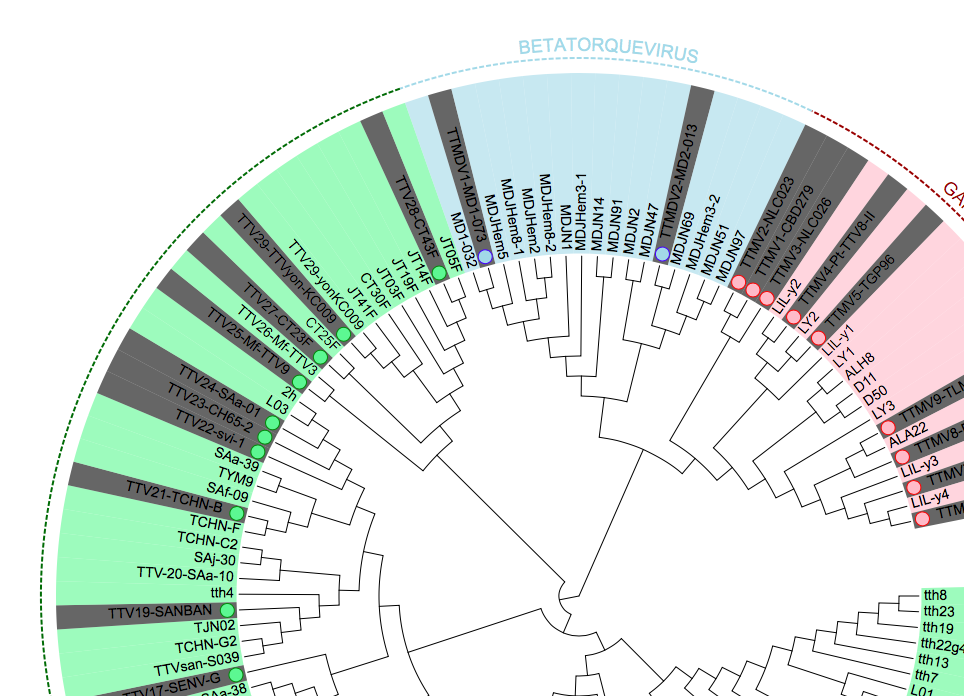
\includegraphics[width=0.7\textwidth,keepaspectratio]{img/mineria/tree2}
%		\label{img:mot2}
%		%\caption{Phylogenetic tree generated by the proposed method. Source: \cite{delibacs2020dna} }
%	\end{figure}
%\end{frame}
%-------------------------------------------------------
%-------------------------------------------------------


%%%%%%%%%%%%%%%%%%%%%%%%%%%%%%%%%%%%%%%%%%%%%%%%%%%%%%%%%%%%%%%%%%%%%%%%%%%%%%%%%%%%%%%%%%%%%%%%%%%%%%%%%%%%%%%%
%%%%%%%%%%%%%%%%%%%%%%%%%%%%%%%%%%%%%%%%%%%%%%%%%%%%%%%%%%%%%%%%%%%%%%%%%%%%%%%%%%%%%%%%%%%%%%%%%%%%%%%%%%%%%%%%
\section{Paper}
%%%%%%%%%%%%%%%%%%%%%%%%%%%%%%%%%%%%%%%%%%%%%%%%%%%%%%%%%%%%%%%%%%%%%%%%%%%%%%%%%%%%%%%%%%%%%%%%%%%%%%%%%%%%%%%%
%%%%%%%%%%%%%%%%%%%%%%%%%%%%%%%%%%%%%%%%%%%%%%%%%%%%%%%%%%%%%%%%%%%%%%%%%%%%%%%%%%%%%%%%%%%%%%%%%%%%%%%%%%%%%%%%

%%%%%%%%%%%%%%%%%%%%%%%%%%%%%%%%%%%%%%%%%%%%%%%%%%%%%%%%%%%%%%%%%%%%%%%%%%%%%%%%%%%%%%%%%%%%%%%%%%%%%%%%%%%%%%%%
%%%%%%%%%%%%%%%%%%%%%%%%%%%%%%%%%%%%%%%%%%%%%%%%%%%%%%%%%%%%%%%%%%%%%%%%%%%%%%%%%%%%%%%%%%%%%%%%%%%%%%%%%%%%%%%%
\subsection{Description}
%%%%%%%%%%%%%%%%%%%%%%%%%%%%%%%%%%%%%%%%%%%%%%%%%%%%%%%%%%%%%%%%%%%%%%%%%%%%%%%%%%%%%%%%%%%%%%%%%%%%%%%%%%%%%%%%
%%%%%%%%%%%%%%%%%%%%%%%%%%%%%%%%%%%%%%%%%%%%%%%%%%%%%%%%%%%%%%%%%%%%%%%%%%%%%%%%%%%%%%%%%%%%%%%%%%%%%%%%%%%%%%%%

%-------------------------------------------------------
%-------------------------------------------------------
\begin{frame}{Paper}{Alignment-free methods}
	\begin{block}{DNA sequence similarity analysis using image texture analysis based	on first-order statistics}
		The authors used \textbf{alignment-free} methods that convert the DNA sequences into feature vectors. They represent DNA sequences as images and then computed the histogram \cite{delibacs2020dna}. 
	\end{block}
\end{frame}
%-------------------------------------------------------
%-------------------------------------------------------

%-------------------------------------------------------
%-------------------------------------------------------
\begin{frame}{Paper}{Image texture analysis}
	\begin{figure}[]
		\centering
		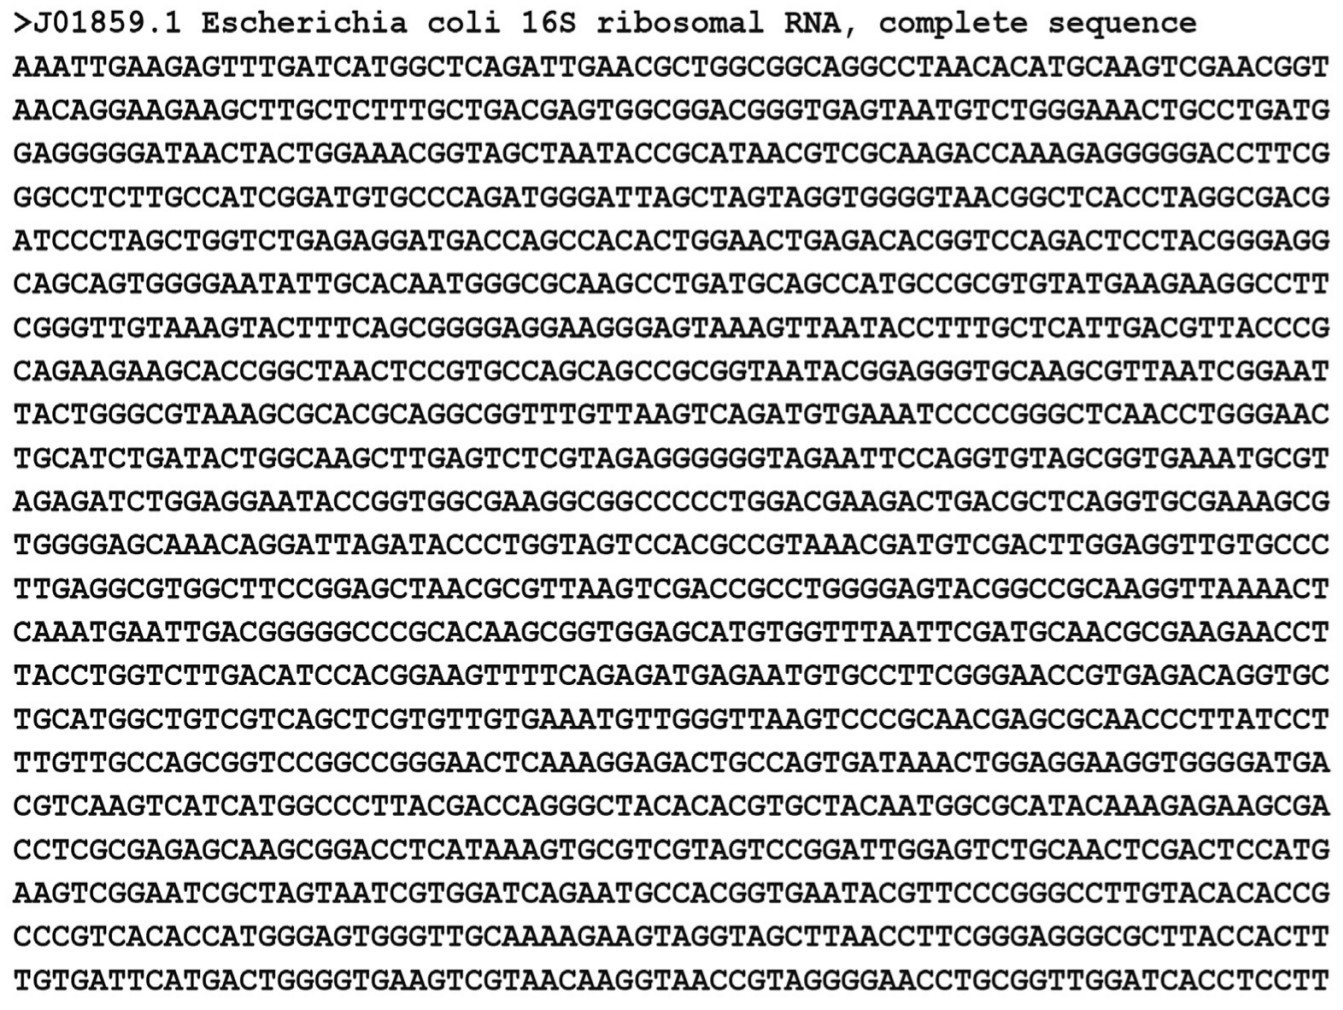
\includegraphics[width=\textwidth,height=0.7\textheight,keepaspectratio]{img/mineria/dnaimg_1}
		\label{img:mot2}
		\caption{16S ribosomal DNA of Escherichia coli with FASTA Format.}
	\end{figure}
\end{frame}
%-------------------------------------------------------
%-------------------------------------------------------

%-------------------------------------------------------
%-------------------------------------------------------
\begin{frame}{Paper}{Image texture analysis}
	\begin{block}{}
		Each pair of bases have a value from $0$ to $15$.
		
		\begin{equation}
			\alpha = \left\lbrace \begin{tabular}{l}
			$AA, AG, AC, AT, GA, GG, GC, GT,$\\
			$CG, CC, CT, CA, TA, TG, TC, TT$
			\end{tabular}      
			  \right\rbrace
		\end{equation}
		
	\end{block}
\end{frame}
%-------------------------------------------------------
%-------------------------------------------------------


%-------------------------------------------------------
%-------------------------------------------------------
\begin{frame}{Paper}{Image texture analysis}
	\begin{figure}[]
		\centering
		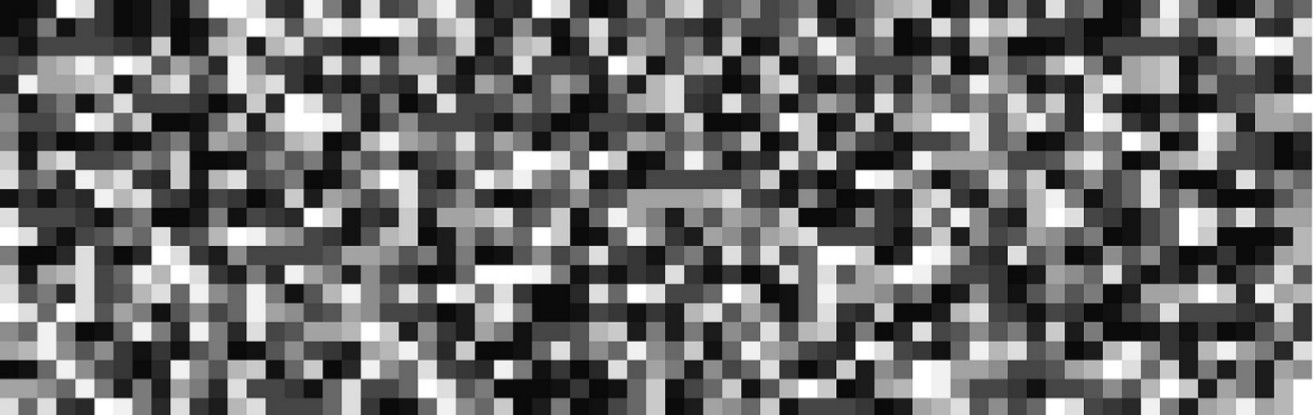
\includegraphics[width=\textwidth,height=0.7\textheight,keepaspectratio]{img/mineria/dnaimg_2}
		\label{img:mot2}
		\caption{Textures converted from the DNA sequences. Source \cite{delibacs2020dna}.}
	\end{figure}
\end{frame}
%-------------------------------------------------------
%-------------------------------------------------------

%-------------------------------------------------------
%-------------------------------------------------------
\begin{frame}{Paper}{Image texture analysis}
	\begin{figure}[]
		\centering
		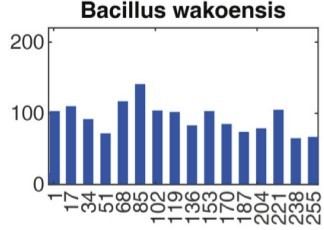
\includegraphics[width=0.6\textwidth,keepaspectratio]{img/mineria/dnaimg_3}
		\label{img:mot2}
		\caption{Histogram of 16S ribosomal DNA. Source \cite{delibacs2020dna}.}
	\end{figure}
\end{frame}
%-------------------------------------------------------
%-------------------------------------------------------

%-------------------------------------------------------
%-------------------------------------------------------
\begin{frame}{Paper}{Image texture analysis}
	\begin{block}{}
		From the histogram, the following features are compute:
		\begin{itemize}
			\item \textbf{\textit{Skewness}} $ = \sigma^{-3} \sum_{i=0}^{G-1} (i - \mu)^3 p(i)$
			\item \textbf{\textit{Kurtosis}} $ = \sigma^{-4} \sum_{i=0}^{G-1} (i - \mu)^4 p(i)-3$
			\item \textbf{\textit{Energy}} $ = \sum_{i=0}^{G-1} p(i)^2$
			\item \textbf{\textit{Entropy}} $ = -\sum_{i=0}^{G-1} p(i)lg(p(i))$
		\end{itemize}
	\end{block}
	
	\begin{block}{}
		Where: 
		\begin{itemize}	
			\item	$p(i) = h(i)/NM$ 
			\item	$h(i) =$ \textit{histogram} 
			\item	$N$ and $M$ \textit{are image's width and height.} 
			\item	$\mu = \sum_{i=0}^{G-1}ip(i)$
		\end{itemize}
	\end{block}
\end{frame}
%-------------------------------------------------------
%-------------------------------------------------------




%%%%%%%%%%%%%%%%%%%%%%%%%%%%%%%%%%%%%%%%%%%%%%%%%%%%%%%%%%%%%%%%%%%%%%%%%%%%%%%%%%%%%%%%%%%%%%%%%%%%%%%%%%%%%%%%
%%%%%%%%%%%%%%%%%%%%%%%%%%%%%%%%%%%%%%%%%%%%%%%%%%%%%%%%%%%%%%%%%%%%%%%%%%%%%%%%%%%%%%%%%%%%%%%%%%%%%%%%%%%%%%%%
\subsection{Results}
%%%%%%%%%%%%%%%%%%%%%%%%%%%%%%%%%%%%%%%%%%%%%%%%%%%%%%%%%%%%%%%%%%%%%%%%%%%%%%%%%%%%%%%%%%%%%%%%%%%%%%%%%%%%%%%%
%%%%%%%%%%%%%%%%%%%%%%%%%%%%%%%%%%%%%%%%%%%%%%%%%%%%%%%%%%%%%%%%%%%%%%%%%%%%%%%%%%%%%%%%%%%%%%%%%%%%%%%%%%%%%%%%


%-------------------------------------------------------
%-------------------------------------------------------
\begin{frame}{Results}{Dataset}
	\begin{table}[]
		\caption{16S ribosomal DNA of 13 bacteria}
		\begin{tabular}{lll}
			\textbf{Specie}                     & \textbf{Accession code} & \textbf{Length(bp) } \\
			\hline
			Bacillus maritimus         & KP317497       & 1515       \\
			Bacillus wakoensis         & NR\_040849     & 1524       \\
			Bacillus australimaris     & NR\_148787     & 1513       \\
			Bacillus xiamenensis       & NR\_148244     & 1513       \\
			Escherichia coli           & J01859         & 1541       \\
			Streptococcus himalayensis & NR\_156072     & 1509       \\
			Streptococcus halotolerans & NR\_152063     & 1520       \\
			Streptococcus tangierensis & NR\_134818     & 1520       \\
			Streptococcus cameli       & NR\_134817     & 1518       \\
			Thermus amyloliquefaciens  & NR\_136784     & 1514       \\
			Thermus tengchongensis     & NR\_132306     & 1523       \\
			Thermus thermophilus       & NR\_037066     & 1515       \\
			Thermus thermophilus       & NR\_117152     & 1514      \\
			\hline
		\end{tabular}
	\end{table}
\end{frame}
%-------------------------------------------------------
%-------------------------------------------------------

%-------------------------------------------------------
%-------------------------------------------------------
\begin{frame}{Results}{Phylogenetic tree}
\begin{figure}[]
	\centering
	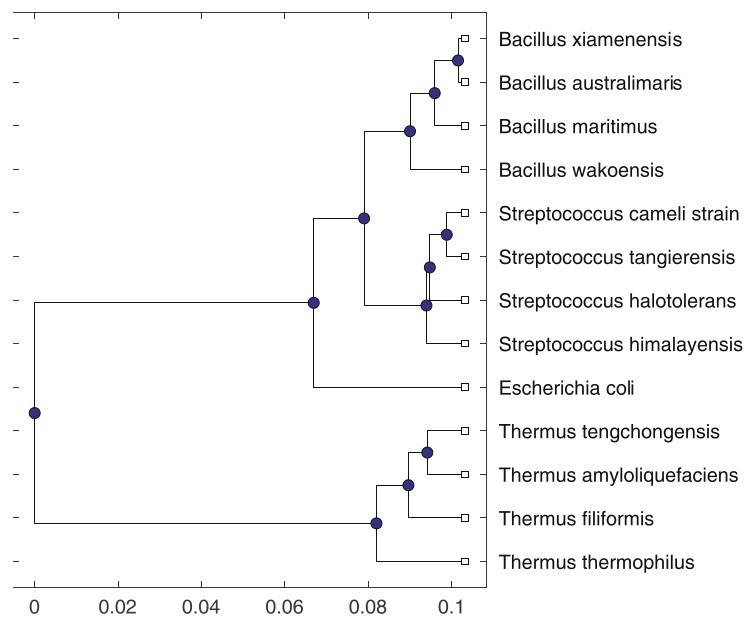
\includegraphics[width=0.7\textwidth,keepaspectratio]{img/mineria/dnaimg_4}
	\label{img:mot2}
	\caption{Phylogenetic tree generated by the proposed method. Source: \cite{delibacs2020dna} }
\end{figure}	
\end{frame}
%-------------------------------------------------------
%-------------------------------------------------------


%-------------------------------------------------------
%-------------------------------------------------------
\begin{frame}{Results}{Phylogenetic tree}
	\begin{figure}[]
		\centering
		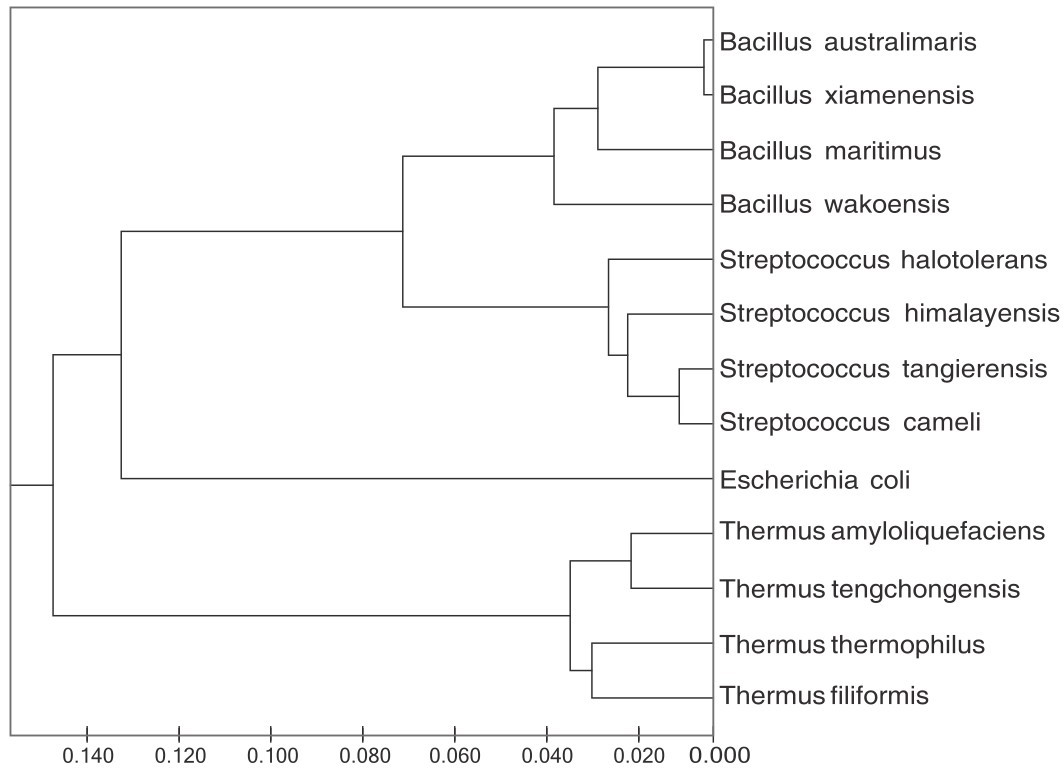
\includegraphics[width=0.8\textwidth,keepaspectratio]{img/mineria/dnaimg_5}
		\label{img:mot2}
		\caption{Phylogenetic tree generated by MEGA7 based on ClustalW alignment and the UPGMA method. Source: \cite{delibacs2020dna} }
	\end{figure}	
\end{frame}
%-------------------------------------------------------
%-------------------------------------------------------


%-------------------------------------------------------
%-------------------------------------------------------
\begin{frame}{Results}{Phylogenetic tree}
	\begin{figure}[]
		\centering
		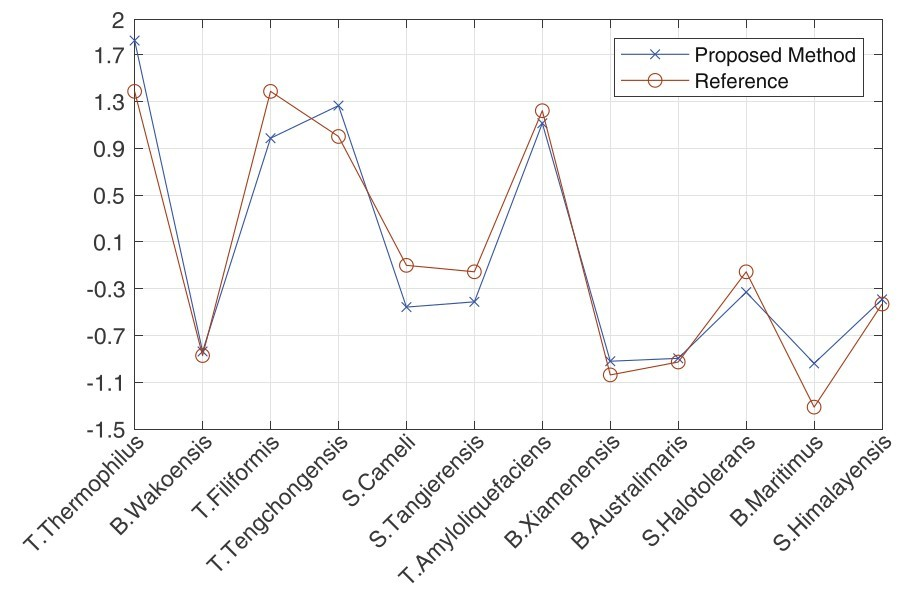
\includegraphics[width=0.8\textwidth,keepaspectratio]{img/mineria/dnaimg_6}
		\label{img:mot2}
		\caption{The degree of similarity/dissimilarity of the other 12 bacteria and Escherichia
			coli. Source: \cite{delibacs2020dna} }
	\end{figure}	
\end{frame}
%-------------------------------------------------------
%-------------------------------------------------------


%%%%%%%%%%%%%%%%%%%%%%%%%%%%%%%%%%%%%%%%%%%%%%%%%%%%%%%%%%%%%%%%%%%%%%%%%%%%%%%%%%%%%%%%%%%%%%%%%%%%%%%%%%%%%%%%
%%%%%%%%%%%%%%%%%%%%%%%%%%%%%%%%%%%%%%%%%%%%%%%%%%%%%%%%%%%%%%%%%%%%%%%%%%%%%%%%%%%%%%%%%%%%%%%%%%%%%%%%%%%%%%%%
\section{Conclusion}
%%%%%%%%%%%%%%%%%%%%%%%%%%%%%%%%%%%%%%%%%%%%%%%%%%%%%%%%%%%%%%%%%%%%%%%%%%%%%%%%%%%%%%%%%%%%%%%%%%%%%%%%%%%%%%%%
%%%%%%%%%%%%%%%%%%%%%%%%%%%%%%%%%%%%%%%%%%%%%%%%%%%%%%%%%%%%%%%%%%%%%%%%%%%%%%%%%%%%%%%%%%%%%%%%%%%%%%%%%%%%%%%%

%-------------------------------------------------------
%-------------------------------------------------------
\begin{frame}{Conclusion}
	\begin{block}{}
		\begin{itemize}
			\item An image texture from DNA is proposed for DNA analysis similarity.
			\item The method proposed results in a phylogenetic tree very similar to the result of MEGA.
			\item The method proposed have a low time processing but the authors did not measure it.
			\item Moreover, It is necessary an evaluation with complete genomes and more samples.
		\end{itemize}
	\end{block}	
\end{frame}
%-------------------------------------------------------
%-------------------------------------------------------



%-------------------------------------------------------
%-------------------------------------------------------
\begin{frame}[allowframebreaks]
\frametitle{References}
%\bibliographystyle{amsalpha}
\bibliographystyle{IEEEtran}
\bibliography{bibliography.bib}
\end{frame}
%-------------------------------------------------------
%-------------------------------------------------------


%-------------------------------------------------------
%-------------------------------------------------------
\if\mycmd1 % MY THEME
	\begin{frame}[plain,noframenumbering]
		%\finalpage{Thank you}
		\begin{figure}[]
			\centering
			
\includegraphics[width=\textwidth,height=0.7\textheight,keepaspectratio]{img/question.png}
			%\label{img:mot2}
			%\caption{Image example in 2 gray levels.}
		\end{figure}
	\end{frame}
	
\else % CS THEME
\begin{frame}{Questions?}
	\begin{figure}[]
		\centering
		
\includegraphics[width=\textwidth,height=0.7\textheight,keepaspectratio]{img/question.png}
		%\label{img:mot2}
		%\caption{Image example in 2 gray levels.}
	\end{figure}
	
\end{frame}
\fi
%-------------------------------------------------------
%-------------------------------------------------------
	
	
\end{document}